\section{Consider the decay at rest \texorpdfstring{$\tau^- \to \pi^- \nu_\tau$}{tau- to pi- nu-tau}, where the spin of the tau is in the positive \texorpdfstring{$z$}{z}-direction and the \texorpdfstring{$\nu_\tau$}{nu-tau} and \texorpdfstring{$\pi^-$}{pi-} travel in the \texorpdfstring{$z$}{z}-directions. Sketch the allowed spin configurations assuming that the form of the weak charged-current interaction is i) V-A and ii) V+A.}

\textbf{i)} In this case, V-A $\implies$ only LH chiral particle states / RH chiral anti-particle states have non-zero projections (the RH particle / LH anti-particle states go to zero). So in our interaction $\tau^- \to \pi^- \nu_\tau$, the neutrino is produced in a LH chiral state. Using the fact that neutrinos are nearly massless, we can say LH chiral $\approx$ LH helicity for the neutrino, which gives us our spin anti-parallel to momentum, as shown on the left.

\textbf{ii)} In this case, we have the opposite thing where only RH particle / LH anti-particle states have non-zero projections $\implies$ RH chiral neutrino $\approx$ RH helicity neutrino $\implies$ spin parallel to momentum.

The question says to make the spin of $\tau$ positive, so that's why 2/4 are crossed out.

\begin{center}
    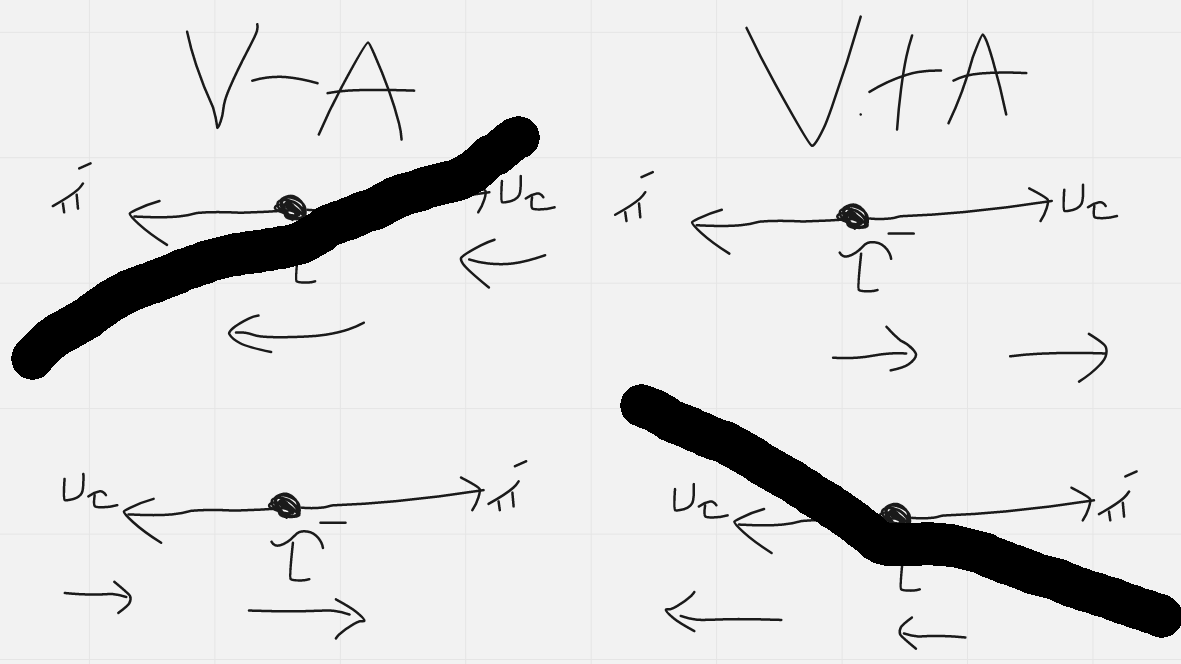
\includegraphics[width=\textwidth]{q1.png}
\end{center}
